\documentclass[14pt]{extarticle} 
\usepackage{amsmath,mathtools,amsfonts,amsthm,amssymb,hyperref}
\usepackage{wasysym,geometry,bussproofs,latexsym,parskip,bookmark}
\usepackage{mathtools,float}
\newtheorem{defn}{Definition}
\newtheorem{thm}{Theorem}
\newtheorem{claim}{Claim}
\newtheorem{lemma}{Lemma}
\newcommand{\dps}{\displaystyle}
\hypersetup{colorlinks,allcolors=blue,linktoc=all}
\geometry{a4paper} 
\geometry{margin=0.5in}
\title{Math for CS 2015/2019 solutions to ``In-Class Problems Week 12, Mon. (Session 28)''}
\author{https://github.com/spamegg1}
\begin{document}
\maketitle
\tableofcontents

\section{Problem 1}
[The Four-Door Deal]

Let’s see what happens when Let’s Make a Deal is played with four doors. A prize is hidden behind one of the four doors. Then the contestant picks a door. Next, the host opens an unpicked door that has no prize behind it. The contestant is allowed to stick with their original door or to switch to one of the two unopened,
unpicked doors. The contestant wins if their final choice is the door hiding the prize.

Let’s make the same assumptions as in the original problem:

1. The prize is equally likely to be behind each door.

2. The contestant is equally likely to pick each door initially, regardless of the prize’s location.

3. The host is equally likely to reveal each door that does not conceal the prize and was not selected by the player.

Use The Four Step Method to find the following probabilities. The tree diagram may become awkwardly large, in which case just draw enough of it to make its structure clear. Also, indicate the set of outcomes in each of the events below. A numerical probability without a demonstration of the Method is not a satisfactory
answer.

\subsection{(a)}
Contestant Stu, a sanitation engineer from Trenton, New Jersey, stays with his original door. What is the probability that Stu wins the prize?
\begin{proof}
??? Do this yourself, it's just repeating the Monty Hall, go through the tree, it's good exercise for you, and way too much work for me to type it here.
\end{proof}

\subsection{(b)}
Contestant Zelda, an alien abduction researcher from Helena, Montana, switches to one of the remaining two doors with equal probability. What is the probability that Zelda wins the prize?
\begin{proof}
??? Do this yourself, it's just repeating the Monty Hall, go through the tree, it's good exercise for you, and way too much work for me to type it here.
\end{proof}

\section{Problem 2}
Suppose there is a system, built by Caltech graduates, with $n$ components. We know from past experience that any particular component will fail in a given year with probability $p$. That is, letting $F_i$ be the event that the ith component fails within one year, we have $Pr[F_i] = p$ for $1 \leq i \leq n$.

The system will fail if any one of its components fails. What can we say about the probability that the system will fail within one year?

Let $F$ be the event that the system fails within one year. Without any additional assumptions, we can’t get an exact answer for $Pr[F]$. However, we can give useful upper and lower bounds, namely,
$$
p \leq Pr[F] \leq np \,\,\,\,\,\,\,\,\,(1)
$$
We may as well assume $p < 1/n$, since the upper bound is trivial otherwise. For example, if $n = 100$ and $p = 10^{-5}$, we conclude that there is at most one chance in 1000 of system failure within a year and at least one chance in 100,000.

Let’s model this situation with the sample space $S \Coloneqq pow([1,n])$ whose outcomes are subsets of positive integers $n$, where $s \in S$ corresponds to the indices of exactly those components that fail within one year. For example, $\{2, 5\}$ is the outcome that the second and fifth components failed within a year and none of the other components failed. So the outcome that the system did not fail corresponds to the empty set, $\emptyset$.

\subsection{(a)}
Show that the probability that the system fails could be as small as $p$ by describing appropriate probabilities for the outcomes. Make sure to verify that the sum of your outcome probabilities is 1.
\begin{proof}
There could be a probability $p$ of system failure if all the individual failures occur to­gether. That is, let 

Pr[$\{1, \ldots , n\}$] $\Coloneqq p$,  Pr[$\emptyset$] $\Coloneqq 1 - p$, and let the probability of all other outcomes be zero. 
So 
$$
F_i = \{s \in S \,\,\,|\,\,\, i \in s\}
$$ 
and 

Pr[$F_i$] $= 0 + 0 + \ldots + 0 \,+ $ Pr[$\{1, \ldots , n\}$] $=$ Pr[$\{1, \ldots , n\}$] $= p$.

Also, the only outcome with positive probability in $F$ is $\{1, \ldots, n\}$, so Pr[$F$] $= p$, as required.
\end{proof}

\subsection{(b)}
Show that the probability that the system fails could actually be as large as $np$ by describing appropriate probabilities for the outcomes. Make sure to verify that the sum of your outcome probabilities is 1.
\begin{proof}
Suppose at most one component ever fails at a time. That is, Pr [$\{i\}$] $= p$ for $1 \leq i \leq n$, Pr[$\emptyset$] $= 1 - np$, and probability of all other outcomes is zero. 

The sum of the probabilities of all the outcomes is one, so this is a well-defined probability space. 

Also, the only outcome in $F_i$ with positive probability is $\{i\}$, so Pr[$F_i$] = Pr[$\{i\}$] $= p$ as required. 

Finally, Pr[$F$] $= np$ because $F = \{A \subseteq \{1, \ldots, n\} \,\,|\,\, A \neq \emptyset\}$, so $F$ in particular contains all the $n$ outcomes of the form $\{i\}$.
\end{proof}

\subsection{(c)}
Prove inequality (1).

\begin{proof}
We will assume the finite version of the Union Bound from Problem 4. (This can also be proved by induction on $n$ and using the 2-event Union Bound in the Induction Step.)

$\dps F = \bigcup_{i=1}^n F_i$, so we have:

\begin{tabular}{rclr}
$p$ & = & Pr[$F_1$] & (given)\\
& $\leq$ & Pr[$F$] & (since $F_1 \subseteq F$)\\
& = & Pr$\left[\dps\bigcup_{i=1}^n F_i\right]$ & (by definition of $F$)\\
& $\leq$ & $\dps\sum_{i = 1}^{n}$Pr[$F_i$]& (Union Bound) \\
& = & $np$ & (since the $F_i$'s are disjoint)
\end{tabular}
\end{proof}

\section{Problem 3}
To determine which of two people gets a prize, a coin is flipped twice. If the flips are a Head and then a Tail, the first player wins. If the flips are a Tail and then a Head, the second player wins. However, if both coins land the same way, the flips don’t count and the whole process starts over.

Assume that on each flip, a Head comes up with probability $p$, regardless of what happened on other flips. Use the four step method to find a simple formula for the probability that the first player wins. What is the probability that neither player wins?

Hint: The tree diagram and sample space are infinite, so you’re not going to finish drawing the tree. Try drawing only enough to see a pattern. Summing all the winning outcome probabilities directly is cumbersome. However, a neat trick solves this problem; and many others. Let $s$ be the sum of all winning outcome probabilities (for the first player) in the whole tree. Notice that you can write the sum of all the winning probabilities (for the first player) in certain subtrees as a function of $s$. Use this observation to write an equation in $s$ and then solve.

\begin{proof} In the tree diagram below, the small triangles represent subtrees that are themselves complete copies of the whole tree.

\begin{figure}[ht!]
\centering
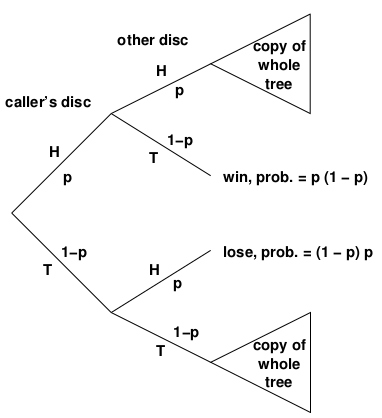
\includegraphics[scale=0.6]{infinite-tree.png}
\end{figure}

Let $s$ equal the sum of all winning probabilities (for the first player) in the whole tree. There are two extra edges with probability $p$ on the path to each outcome in the top subtree. Therefore, the sum of winning probabilities in the upper copy-subtree is $p^2 s$. Similarly, the sum of winning probabilities in the lower copy-subtree is $(1 - p)^2s$. This gives the equation:

$$
s = p^2s + (1-p)^2s + p(1-p)
$$

The solution to this equation is $s = 1/2$, for all $p$ between $0$ and $1$.

By symmetry, the probability that the first player loses is 1/2. This means that the event, if any, of flipping forever can only have probability zero.

Formally, the sample space is the (infinite) set of leaves of the tree, namely,

$$
S \Coloneqq \{TT, HH\}^* \cdot \{HT, TH\}
$$

where $\{TT, HH\}^*$ denotes the set of strings formed by concatenating a sequence of $HH$s and $TT$s. For example,

$$
TTTTHHHT, HHTTTH, HHHHHHHHHT, HT \in S
$$

For any string $s \in S$ we have

$$
\text{Pr}[s] \Coloneqq p^{\text{\# H's in }s}(1-p)^{\text{\# T's in }s}
$$

To verify that is defines a probability space, we must show that $\sum_{s \in S}Pr[s] = 1$.

\begin{tabular}{rclr}
$\dps\sum_{s \in S}$Pr[$s$] &=& $\dps\sum_{n \geq 0} \sum_{s \in S, |s| = 2n+2} p^{\text{\# H's in }s}(1-p)^{\text{\# T's in }s}$ &\\
&=& $\dps\sum_{n \geq 0} \sum_{i+j=n} p^{2i}(1-p)^{2j}p(1-p)$ & (strings that end in HT)\\
& & $\dps + \sum_{n \geq 0} \sum_{i+j=n} p^{2i}(1-p)^{2j}p(1-p)$ & (strings that end in TH)\\
&=& $\dps 2p(1-p)\sum_{n \in \mathbb{N}}(p^2 + (1-p)^2)^n $ & \\
&=& $\dps \frac{2p(1-p)}{1 - (p^2 + (1-p)^2)}$ & \\
&=& $\dps \frac{2p(1-p)}{-2p^2+2p}$ & \\
&=& 1 & \\
\end{tabular}

\end{proof}

\section{Problem 4}
Prove the following probabilistic inequality, referred to as the Union Bound. Let $A_1, \ldots, A_n, \ldots$ be events. Then
$$
Pr\left[\bigcup_{n \in \mathbb{N}}A_n\right] \leq \sum_{n \in \mathbb{N}}Pr[A_n]
$$
Hint: Replace the $A_n$’s by pairwise disjoint events and use the Sum Rule.

\begin{proof}
Define $B_1 \Coloneqq A_1$ and for all $j \geq 2$ define
$$
B_j \Coloneqq A_j - \bigcup_{i = 1}^{j-1} A_i
$$
Then all the $B_j$s are pairwise disjoint, and
$$
\bigcup_{n \in \mathbb{N}} B_n = \bigcup_{n \in \mathbb{N}} A_n
$$
By the Disjoint Sum Rule (this is an infinite series, but it's justified: we know the infinite series converges because it's bounded above by 1, and has nonnegative terms):
$$
Pr\left[\bigcup_{n \in \mathbb{N}} B_n\right] = \sum_{n \in \mathbb{N}} \text{Pr}[B_n]
$$
For all $n \in \mathbb{N}$ we have $B_n \subseteq A_n$, so by Monotonicity (below)
$$
\text{Pr}[B_n] \leq \text{Pr}[A_n]
$$
Combining all these facts, we obtain
$$
Pr\left[\bigcup_{n \in \mathbb{N}}A_n\right] = Pr\left[\bigcup_{n \in \mathbb{N}}B_n\right] = \sum_{n \in \mathbb{N}} \text{Pr}[B_n] \leq \sum_{n \in \mathbb{N}} \text{Pr}[A_n]
$$
\end{proof}

\section{Problem 5 (Supplemental Problem)}
Here are some handy rules for reasoning about probabilities that all follow directly from the Disjoint Sum Rule. Prove them.

\subsection{(a)}
Pr[$A - B$] = Pr[$A$] $-$ Pr[$A \cap B$] (Difference Rule)
\begin{proof}
Any set $A$ is the disjoint union of $A - B$ and $A \cap B$, so by the Disjoint Sum Rule: Pr[$A$] = Pr[$A - B$] $+$ Pr[$A \cap B$]. Then we can rearrange the terms to prove the Difference Rule.
\end{proof}

\subsection{(b)}
Pr[$\overline{A}$] = 1 $-$ Pr[$A$] (Complement Rule)
\begin{proof}
We have $\overline{A} \Coloneqq S - A$ (where $S$ is the sample space of all outcomes, so Pr[$S$] = 1), so we can apply the Difference Rule (which we just proved above): Pr[$\overline{A}$] = Pr[$S$] $-$ Pr[$A$] = 1 $-$ Pr[$A$].
\end{proof}

\subsection{(c)}
Pr[$A \cup B$] = Pr[$A$] $+$ Pr[$B$] $-$ Pr[$A \cap B$] (Inclusion-Exclusion)

\begin{proof}
$A \cup B$ is the disjoint union of $A$ and $B - A$, so by the Disjoint Sum Rule we have Pr[$A \cup B$] = Pr[$A$] $+$ Pr[$B - A$].

Now apply the Difference Rule to the second term: Pr[$B - A$] = Pr[$B$] $-$ Pr[$A \cap B$]. Using this above, we get: Pr[$A \cup B$] = Pr[$A$] $+$ Pr[$B$] $-$ Pr[$A \cap B$].
\end{proof}

\subsection{(d)}
Pr[$A \cup B$] $\leq$ Pr[$A$] + Pr[$B$] (2-event Union Bound)

\begin{proof}
By Inclusion-Exclusion (which we just proved above): Pr[$A \cup B$] = Pr[$A$] $+$ Pr[$B$] $-$ Pr[$A \cap B$].

Now we have Pr[$A \cap B$] $\geq 0$ by definition of probability. Therefore Pr[$A \cup B$] = Pr[$A$] $+$ Pr[$B$] $-$ Pr[$A \cap B$] $\leq$ Pr[$A$] $+$ Pr[$B$].
\end{proof}

\subsection{(e)}
If $A \subseteq B$ then Pr[$A$] $\leq$ Pr[$B$] (Monotonicity)

\begin{proof}
Notice that since $A \subseteq B$ we have $A \cap B = A$. So:

\begin{tabular}{rclr}
Pr[$B$]&=&Pr[$B$] $-$ (Pr[$B$] $-$ Pr[$A$])&\\
&=&Pr[$B$] $-$ (Pr[$B$] $-$ Pr[$A \cap B$])& (since $A = A \cap B$)\\
&=&Pr[$B$] $-$ (Pr[$B-A$])& (Difference Rule)\\
&=&Pr[$B$]& (since Pr[$B-A$] $\geq 0$)
\end{tabular}
\end{proof}

\section{Problem 6 (Supplemental Problem)}
The New York Yankees and the Boston Red Sox are playing a two-out-of-three series. In other words, they play until one team has won two games. Then that team is declared the overall winner and the series ends. Assume that the Red Sox win each game with probability 3/5, regardless of the outcomes of previous games.

Answer the questions below using the four step method. You can use the same tree diagram for all three problems.

\begin{figure}[ht!]
\centering
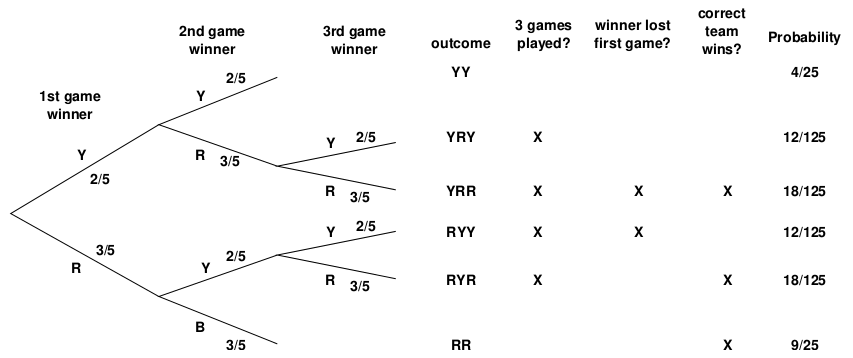
\includegraphics[scale=0.6]{red-sox.png}
\end{figure}

\subsection{(a)}
What is the probability that a total of 3 games are played?
\begin{proof}
From the tree diagram we get
$$
\text{Pr[3 games played]} = \frac{12}{125} + \frac{18}{125} + \frac{12}{125} + \frac{18}{125} = \frac{60}{125}
$$
\end{proof}

\subsection{(b)}
What is the probability that the winner of the series loses the first game?
\begin{proof}
From the tree diagram we get
$$
\text{Pr[winner lost first game]} = \frac{18}{125} + \frac{12}{125}  = \frac{30}{125}
$$
\end{proof}

\subsection{(c)}
What is the probability that the correct team wins the series?
\begin{proof}
From the tree diagram we get
$$
\text{Pr[correct team wins]} = \frac{18}{125} + \frac{18}{125} + \frac{45}{125} = \frac{81}{125}
$$
\end{proof}

\end{document}
